%%*****************************************************************************
%%  METHODOLOGY
%%
%%  MIGRATED FROM THE IEEE-FORMAT PROPOSAL. The wording below is UNCHANGED
%%  from the proposal except for the mechanical conversions listed here:
%%    - \section -> \chapter, \subsection -> \section, etc. (one level up)
%%    - \columnwidth -> \linewidth (the book class is single column)
%%    - figure paths now resolve through \graphicspath below
%%    - IEEE two-column spacing crutches removed (\hspace*{1.5em} paragraph
%%      indents and \vspace{0.5\baselineskip} gaps); the book class indents
%%      and spaces paragraphs on its own
%%
%%  STILL TO DO IN THIS FILE - see MIGRATION-NOTES.md:
%%    1. TENSE PASS. This chapter is the most affected: it describes a system
%%       that did not exist yet and now does.
%%    2. Maam Antoi named this chapter specifically as needing rewriting
%%       because the proposal version is generic.
%%    3. CORRECTIONS OVERDUE (see MIGRATION-NOTES.md for the full table):
%%       growing medium, 13 cm pots not 200 mm, Camera Module 3 not V2,
%%       array geometry, always-on power not deep-sleep, enclosure material
%%       and dimensions, and the per-pot area measure.
%%    4. MISSING SECTION: the panel asked how the camera data is validated.
%%       Section 'System Calibration and Pre-Deployment Validation' has five
%%       items and every one validates the apparatus, not the measurement.
%%       Add a sixth: GPR validation against hand-labelled ground truth.
%%*****************************************************************************

\chapter{Methodology}
\label{chap:methodology}

\ifpdf
    \graphicspath{{Chapter3/Figs/Raster/}{Chapter3/Figs/PDF/}{Chapter3/Figs/}}
\else
    \graphicspath{{Chapter3/Figs/Vector/}{Chapter3/Figs/}}
\fi

\section{Experimental Design and Agronomic Controls}

This study implements a structured quantitative experimental design to evaluate a computer vision architecture for non-destructive yield estimation. The cultivation trials focus on Pechay (\textit{Brassica rapa}) observed over a standard 35-day vegetative grow-out cycle, which falls within the documented 30- to 45-day harvest window for the crop \cite{Camariosa2021}. To isolate the primary mathematical relationship between daily extracted visual canopy features and final fresh-weight biomass at harvest, strict agronomic control variables are maintained within a controlled greenhouse setting:

\textbf{Cultivation Timeline and Day Indexing.} The growth cycle index \(D\) is defined such that \(D = 1\) corresponds to the date of direct seed sowing into the final container, consistent with the direct-sowing protocol employed in the prior institutional deployment \cite{ZamoraOgue2025}. Seedling emergence is expected between \(D = 5\) and \(D = 7\). Physical harvest and ground-truth fresh-weight measurement are performed on \(D = 35\), on the same day as and immediately following the final scheduled image capture, so that the terminal point of each GPR time-series corresponds temporally to the measured harvest weight. This alignment is a deliberate methodological refinement: in the prior institutional deployment, growth observation concluded on day 37 while harvest was performed on day 44, with manual watering applied during the intervening period \cite{ZamoraOgue2025}, which decoupled the final recorded growth state from the measured harvest mass.

\begin{enumerate}
    \item \textbf{Substrate Uniformity:} All specimens are cultivated in individual, structurally isolated containers using uniform Department of Agriculture (DA) soil media composed of loam, organic compost, and carbonized rice husk. To guarantee substrate consistency and eliminate chemical variability, a manual spot-check of the soil pH baseline is conducted using a calibrated manual tester at Day 0 of the planting cycle, establishing a stable starting chemistry profile across all nodes.
    \item \textbf{Root Isolation:} Isolating each plant into an individual pot container strictly bounds the rooting volume and neutralizes inter-specimen root-zone competition for localized water, space, and macronutrients.
    \item \textbf{Differential Moisture Control:} The inherited 1:1 solenoid-based micro-irrigation system \cite{ZamoraOgue2025} is configured to maintain three independent soil moisture treatment groups across the 9 container pots: Group A (Low: 30-40\% VWC), Group B (Optimal: 50-60\% VWC), and Group C (High: 70-80\% VWC). This autonomous baseline ensures strict root-zone moisture regulation without any manual watering intervention, while providing necessary variance for the multivariate prediction model. Any departure from this autonomous regime is recorded and disclosed as a logged deviation in accordance with the constraints stated in Section I.G.
\end{enumerate}

\section{Physical Cultivation Geometry and Spatial Setup}

To ensure consistent digital image acquisition and eliminate microclimatic or visual cross-contamination between specimens, the physical cultivation framework is organized according to strict spatial dimensions.

\textbf{1) Container Pot Specifications:} All nine experimental units utilize identical cylindrical polyethylene container pots featuring an upper diameter of $200\,\mathrm{mm}$ ($20\,\mathrm{cm}$), a base diameter of $130\,\mathrm{mm}$ ($13\,\mathrm{cm}$), and a vertical depth of $200\,\mathrm{mm}$ ($20\,\mathrm{cm}$). Each container holds approximately $3.0\,\mathrm{L}$ of standardized Department of Agriculture (DA) bulk soil medium, providing sufficient volume for unrestricted root development without inducing pot-bound stress during the 35-day grow-out cycle.

\textbf{2) Grid Array and Inter-Pot Clearance:} The nine pots are positioned on a planar cultivation bench arranged in a uniform $3 \times 3$ grid array. A standardized edge-to-edge clearance of $150\,\mathrm{mm}$ ($15\,\mathrm{cm}$) is maintained between adjacent pots, establishing a center-to-center pitch of $350\,\mathrm{mm}$ ($35\,\mathrm{cm}$). This spatial buffer provides two essential experimental controls:
\begin{itemize}
    \item \textit{Agronomic Isolation:} It prevents mature vegetative canopies (typical maximum spread of $180\text{--}220\,\mathrm{mm}$ at harvest) from physically touching or shading neighboring specimens, guaranteeing independent light capture across treatment groups.
    \item \textit{Vision Segmentation Integrity:} It creates a wide, high-contrast soil/space margin around each pot perimeter, allowing the digital Region of Interest (ROI) bounding boxes (\texttt{pot\_rois.json}) to crop individual plant canopies cleanly without leaf intrusion from adjacent pots.
\end{itemize}

\textbf{3) Camera Mounting Elevation and Field of View (FOV):} A single Raspberry Pi Camera Module V2 (8-Megapixel, $62.2^\circ$ horizontal FOV, $48.8^\circ$ vertical FOV) is mounted overhead above the pot rim plane at a nominal elevation of approximately $1100\,\mathrm{mm}$ ($110\,\mathrm{cm}$), oriented at a true $90^\circ$ perpendicular angle (nadir view). With a center-to-center pitch of $350\,\mathrm{mm}$ and a pot rim diameter of $200\,\mathrm{mm}$, the full $3 \times 3$ array occupies a square footprint of $900\,\mathrm{mm} \times 900\,\mathrm{mm}$. Because the sensor's vertical field of view is narrower than its horizontal field of view, the vertical dimension governs the minimum required elevation: coverage of the $900\,\mathrm{mm}$ span requires a height of at least $992\,\mathrm{mm}$, and the nominal $1100\,\mathrm{mm}$ elevation yields a coverage area of approximately $1327\,\mathrm{mm} \times 998\,\mathrm{mm}$, providing a margin of roughly $49\,\mathrm{mm}$ on each edge against mounting tolerance. At this elevation the imaged ground resolution remains approximately $24.7$ pixels per centimetre, so an individual pot rim spans on the order of $490$ pixels, which is substantially finer than the precision required for Green Pixel Ratio extraction. This elevation is treated as a design target; the final mounting height is empirically established and locked during pre-deployment calibration, as described in Section III.E.

\begin{figure}[htbp]
    \centering
    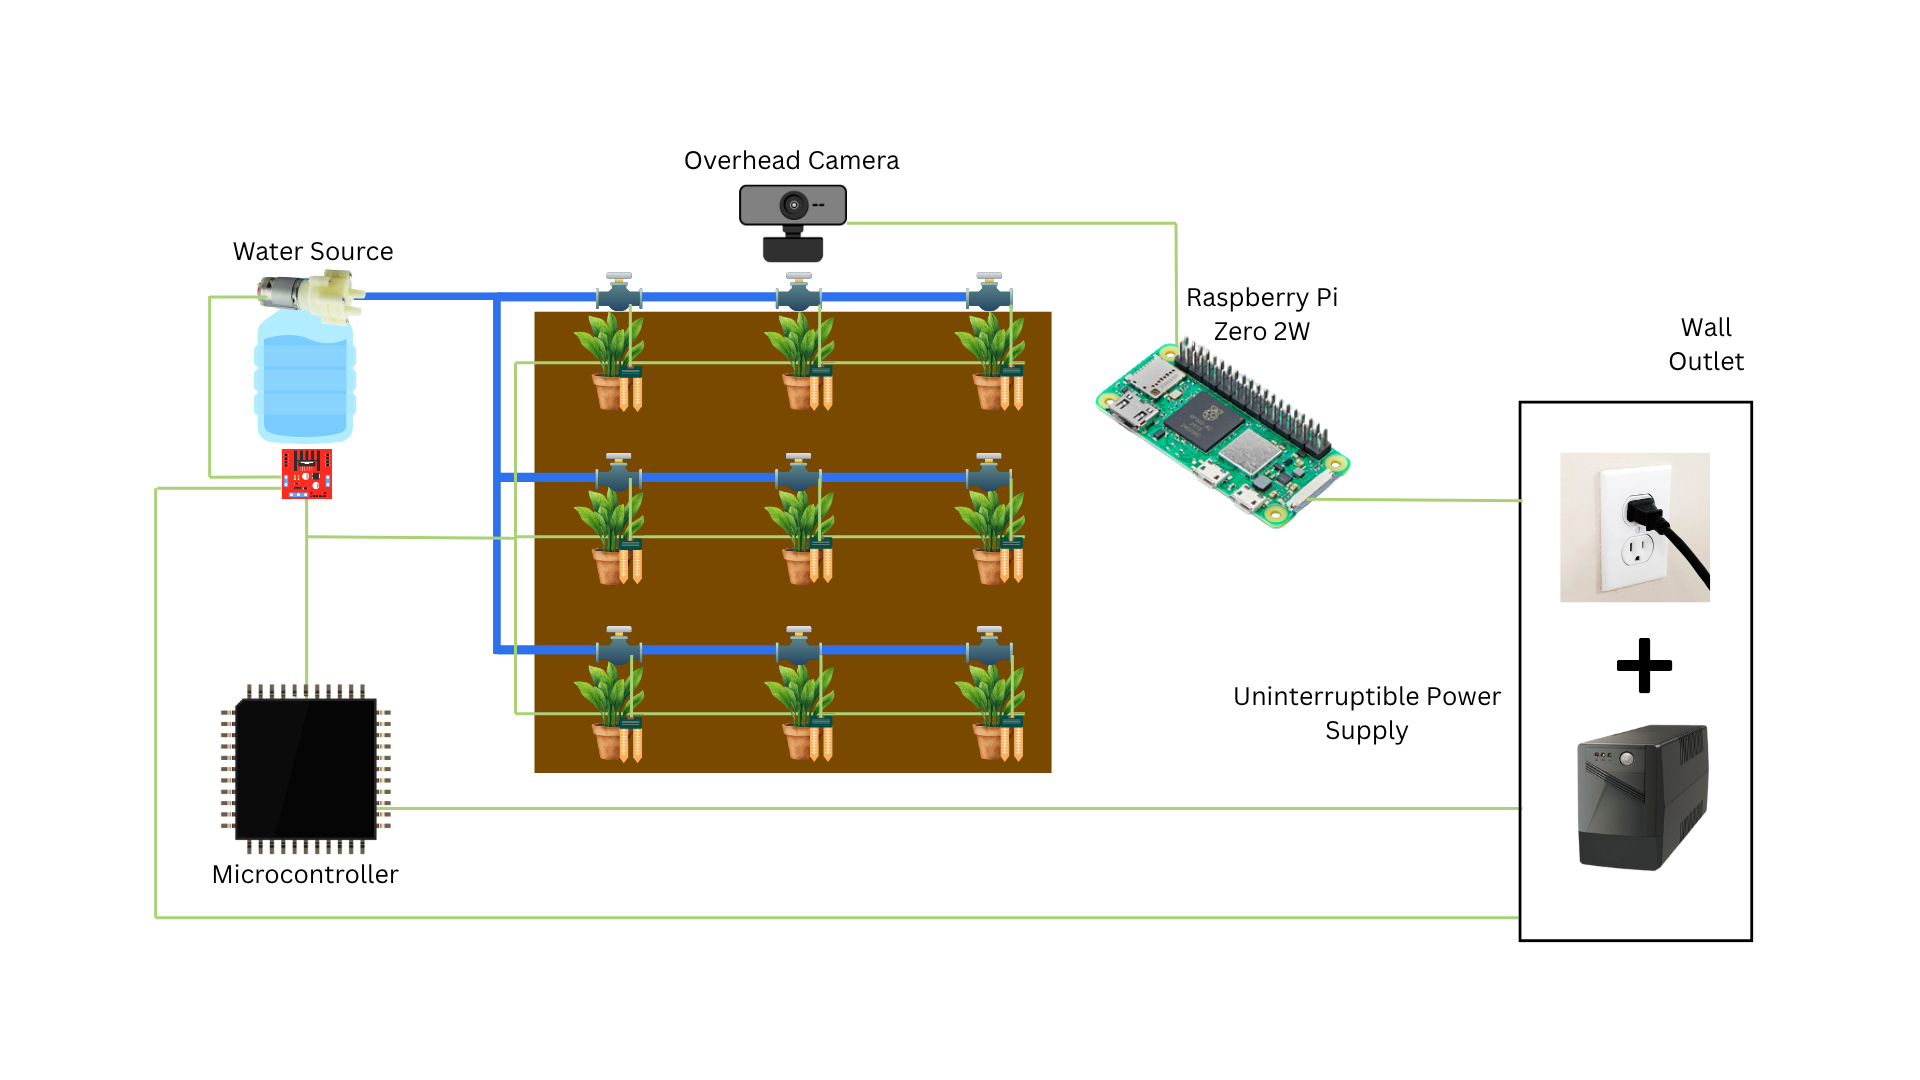
\includegraphics[width=0.85\linewidth]{PhysicalSetup.png}
    \caption{Physical setup of the greenhouse cultivation system showing the overhead camera, Raspberry Pi Zero 2W, microcontroller, water source, irrigation lines, 9-pot planting layout, and UPS-backed wall power connection.}
    \label{fig:physical-setup-ups}
\end{figure}

\section{Stage 1: Physical System Stabilization and Interconnect Isolation}

Building upon the previous institutional lineage \cite{ZamoraOgue2025}, the physical hardware framework is modified exclusively to secure signal telemetry integrity against the high-humidity conditions of a greenhouse microclimate. Unstructured copper core jumper wire matrices are eliminated and replaced by a unified, custom-designed Printed Circuit Board (PCB) routing interface. The custom PCB houses all signal routing paths, grouping capacitive soil moisture sensor lines and minimizing inductive loop areas.

The capacitive sensor probe blades inserted within the soil substrate require robust environmental protection to maintain long-term calibration and prevent hardware degradation. Prior institutional implementations utilizing exposed sensors within similar humid greenhouse environments experienced significant physical deterioration and subsequently transmitted erroneous moisture data \cite{ZamoraOgue2025}. To mitigate this vulnerability, an industrial-grade conformal coating is applied to the sensor PCB assemblies. This specialized coating creates a physical hydrophobic barrier that neutralizes atmospheric moisture ingress and prevents copper trace deterioration, ensuring reliable dielectric permittivity measurements without distorting the underlying electronic characteristics of the sensor in accelerated tropical environments \cite{Sheng2019}.

\section{Stage 2: Overhead Single-Camera Visual Acquisition Pipeline}

The visual data acquisition node is optimized to extract structural canopy metrics while minimizing hardware footprint. A single high-resolution camera module is mounted directly above each cultivation vessel at a strict \(90^{\circ}\) perpendicular angle (nadir view). This positioning provides a flat, two-dimensional coordinate space that maps pixel area uniformly to growth area, significantly minimizing perspective warp and leaf occlusion. The visual data acquisition process follows a scheduled sequence managed collaboratively by the primary controllers:

\begin{enumerate}
    \item \textbf{Always-On Scheduled Capture:} To mitigate boot-cycle hardware failures and file-system corruption associated with hard power-cycling, the Raspberry Pi Zero 2W operates in a headless, always-on state. Image capture is executed autonomously via a \texttt{cron}-scheduled Python script configured to trigger daily at 12:00 PM (noon) under uniform greenhouse LED illumination.
    \item \textbf{Live-Feed Frame Sampling:} Upon execution, the Python script opens a continuous live video stream from the camera and allows the sensor's automatic exposure and white balance to stabilize over a brief warm-up interval. A single representative uncompressed nadir frame is then sampled from the live feed, written to local memory, and the stream is released. Sampling a stabilized frame from a live feed, rather than performing a cold single-shot capture, improves exposure consistency and optical stability across the daily image series.
    \item \textbf{Digital Masking and Smoothing:} To secure illumination invariance, frames undergo localized transformation into the Hue-Saturation-Value (HSV) color space with an empirically calibrated Hue mask (\(35^{\circ} \leq \text{Hue} \leq 85^{\circ}\)). To prevent background noise from adjacent overlapping leaves or structural borders, the pipeline utilizes a fixed JSON configuration file (\texttt{pot\_rois.json}) to apply targeted Region of Interest (ROI) bounding boxes, isolating the GPR computation strictly to individual pot perimeters. The computed daily GPR percentage is logged locally to a CSV file.
    \item \textbf{Handling of Overlapping Canopy Pixels:} As the canopy expands toward closure, leaves may extend laterally beyond the pot rim. The pipeline enforces a strict spatial attribution rule: every pixel satisfying the green threshold within a given pot's ROI is attributed to that pot, and any pixel falling outside the ROI is discarded irrespective of the specimen from which it originates. The ROI boundary for each pot is inscribed within the pot rim with a guard margin, and the inter-pot clearance specified in Section III.B is selected so that lateral canopy extension remains smaller than the distance between adjacent ROI boundaries for the duration of the cycle. A morphological opening operation is applied to the binary mask prior to pixel counting in order to sever thin leaf bridges that may momentarily span adjacent regions. Any acquisition day on which canopy encroachment across an ROI boundary is observed is flagged in the anomaly log and reported with the results.
    \item \textbf{Data Interpolation (Offline):} To mathematically smooth transient daily anomalies (e.g., wind-induced leaf shifting or temporary shadows) and address potential single-day capture failures, a 3-day centered moving average is applied to each plant's complete GPR time-series. Because a centered average requires observations from days both before and after each point, this smoothing is performed offline (post hoc) during the analysis stage after the full grow-out is complete, and not within the daily cron routine, which logs only the raw per-day GPR value. Raw image payloads are systematically purged from disk storage after each daily data extraction to enforce storage autonomy.
\end{enumerate}

\begin{figure}[htbp]
    \centering
    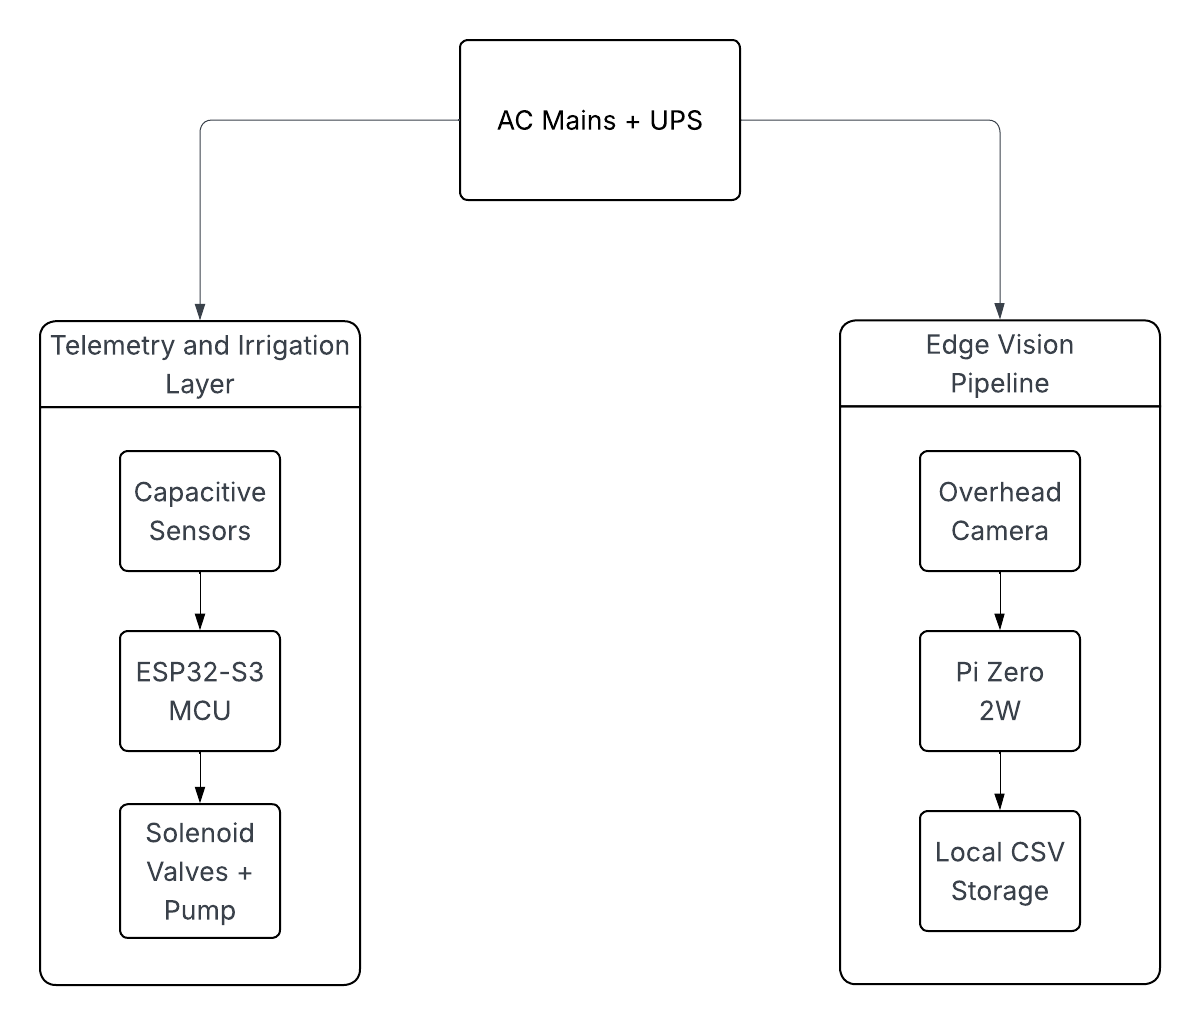
\includegraphics[width=\linewidth]{In-text_SystemArchitecture.png}
    \caption{System architecture detailing the separation of the ESP32 baseline irrigation logic and the Raspberry Pi Zero 2W vision pipeline.}
    \label{fig:methodology_flowchart}
\end{figure}

\section{System Calibration and Pre-Deployment Validation}
\label{sec:calibration}

Prior to the execution of the full 35-day biological grow-out cycle, the decoupled architecture undergoes strict pre-deployment testing to establish empirical baselines and guarantee data integrity.

\begin{enumerate}
    \item \textbf{Sensor Calibration and Differential Irrigation Tuning:} The custom-coated capacitive soil moisture sensors are calibrated using a two-point extreme baseline method (bone-dry vs. fully saturated DA soil). These extremes map the functional ADC boundaries, allowing the ESP32-S3 to reliably enforce the three distinct treatment thresholds (30-40\%, 50-60\%, and 70-80\% VWC) across the respective pot groups.
    \item \textbf{Cron Execution and Storage Autonomy Testing:} The vision processing node undergoes an isolated 72-hour continuous uptime test to verify the reliability of the headless architecture. This validates that the \texttt{cron}-scheduled Python script successfully triggers at exactly 12:00 PM, captures the image, executes the ROI mask and HSV extraction, saves the CSV data, and successfully deletes the raw image payload to prevent storage overflow.
    \item \textbf{Illumination and HSV Tuning:} To prevent background noise from corrupting the daily GPR extraction, the OpenCV HSV threshold parameters are fine-tuned. Testing is conducted strictly under the activated greenhouse LED enclosure using sample Pechay leaves. This visual calibration ensures the binarization mask (\(35^{\circ} \leq \text{Hue} \leq 85^{\circ}\)) cleanly isolates vegetative tissue while actively rejecting soil artifacts, pot boundaries, and LED glare.
    \item \textbf{Camera Field-of-View and ROI Mapping Calibration:} Before the official grow-out cycle commences, empirical testing establishes the optimal vertical elevation of the camera rig. The physical height is adjusted to capture the full array of pots, and the digital bounding coordinates for each of the 9 pots are finalized and locked into the \texttt{pot\_rois.json} configuration file to ensure GPR calculations strictly isolate the internal pot surface area. The nominal elevation of approximately $1100\,\mathrm{mm}$ specified in Section III.B serves as the starting point for this adjustment.
    \item \textbf{Canopy Overlap and ROI Boundary Validation:} The spatial attribution rule defined in Section III.D is validated prior to deployment by positioning mature Pechay leaf samples so that they span the boundary between adjacent pot regions, confirming that pixels lying outside a given ROI are correctly excluded from that pot's computation and that the morphological opening operation severs artificial leaf bridges as specified. Canopy extent relative to the ROI boundary is subsequently re-examined during each weekly inspection, and the acquisition date on which any canopy first approaches its ROI boundary is recorded for reference during analysis.
\end{enumerate}

\section{Stage 3: Predictive Modeling Formulation and Verification}

At the termination of the 35-day cultivation cycle, the cumulative time-series CSV logs for all 9 plants are extracted. Ground-truth above-ground fresh-weight biomass (\(Y\), measured in grams) is recorded for each specimen using a calibrated digital scale at the precise point of physical harvest.

Crop growth is fundamentally a nonlinear process: canopy expansion and biomass accumulation follow a sigmoidal trajectory of slow initial establishment, near-exponential mid-cycle expansion, and a late-cycle plateau as canopy closure and self-shading limit further gain \cite{Archontoulis2015}. Rather than committing the model to a single parametric growth form such as the logistic or Gompertz function, this study adopts a second-degree multivariate polynomial as a flexible local approximation of the underlying nonlinear yield-response surface that remains linear in its parameters and is therefore estimable by ordinary least squares. To guard against overfitting, the specification is kept deliberately parsimonious. Although the pooled dataset contains 315 daily rows, the effective sample for generalization is the nine independent plants evaluated under leave-one-plant-out cross-validation, and established guidance recommends on the order of 10--15 observations per estimated parameter to obtain stable coefficients \cite{Harrell2015}. The eight-term specification is accordingly reduced to six terms: because the Green Pixel Ratio rises monotonically with day-in-cycle \(D\) during vegetative growth, \(D\) and \(GPR\) are strongly collinear, so the \(D^2\) and \(D \times GPR\) terms are removed to suppress the resulting multicollinearity, while \(D\) is retained as a linear growth-stage covariate and the well-identified \(GPR^2\) curvature and \(GPR \times SM\) interaction are preserved.

Unlike single-variable estimators, this study utilizes a multivariate polynomial regression framework to account for the interacting effects of structural canopy size, biological age, and soil moisture availability. The final dataset comprises 315 total observations (9 plants \(\times\) 35 days). The predictive model maps the independent variables directly against the final harvest weight using a 6-term polynomial equation:

\begin{equation}
\begin{aligned}
\hat{Y} = & \beta_0 + \beta_1D + \beta_2GPR + \beta_3SM \\
& + \beta_4GPR^2 + \beta_5(GPR \times SM) + \varepsilon
\end{aligned}
\tag{1}
\end{equation}

where:
\begin{itemize}
    \item \(\hat{Y}\) = Predicted final fresh-weight biomass at harvest (grams)
    \item \(D\) = Day in the growth cycle (1 through 35)
    \item \(GPR\) = Green Pixel Ratio (percentage of canopy cover)
    \item \(SM\) = Volumetric Water Content (percentage from the capacitive sensor)
    \item \(\beta_0 \dots \beta_5\) = The learned regression coefficients
    \item \(\varepsilon\) = The error term
\end{itemize}

\begin{figure}[htbp]
    \centering
    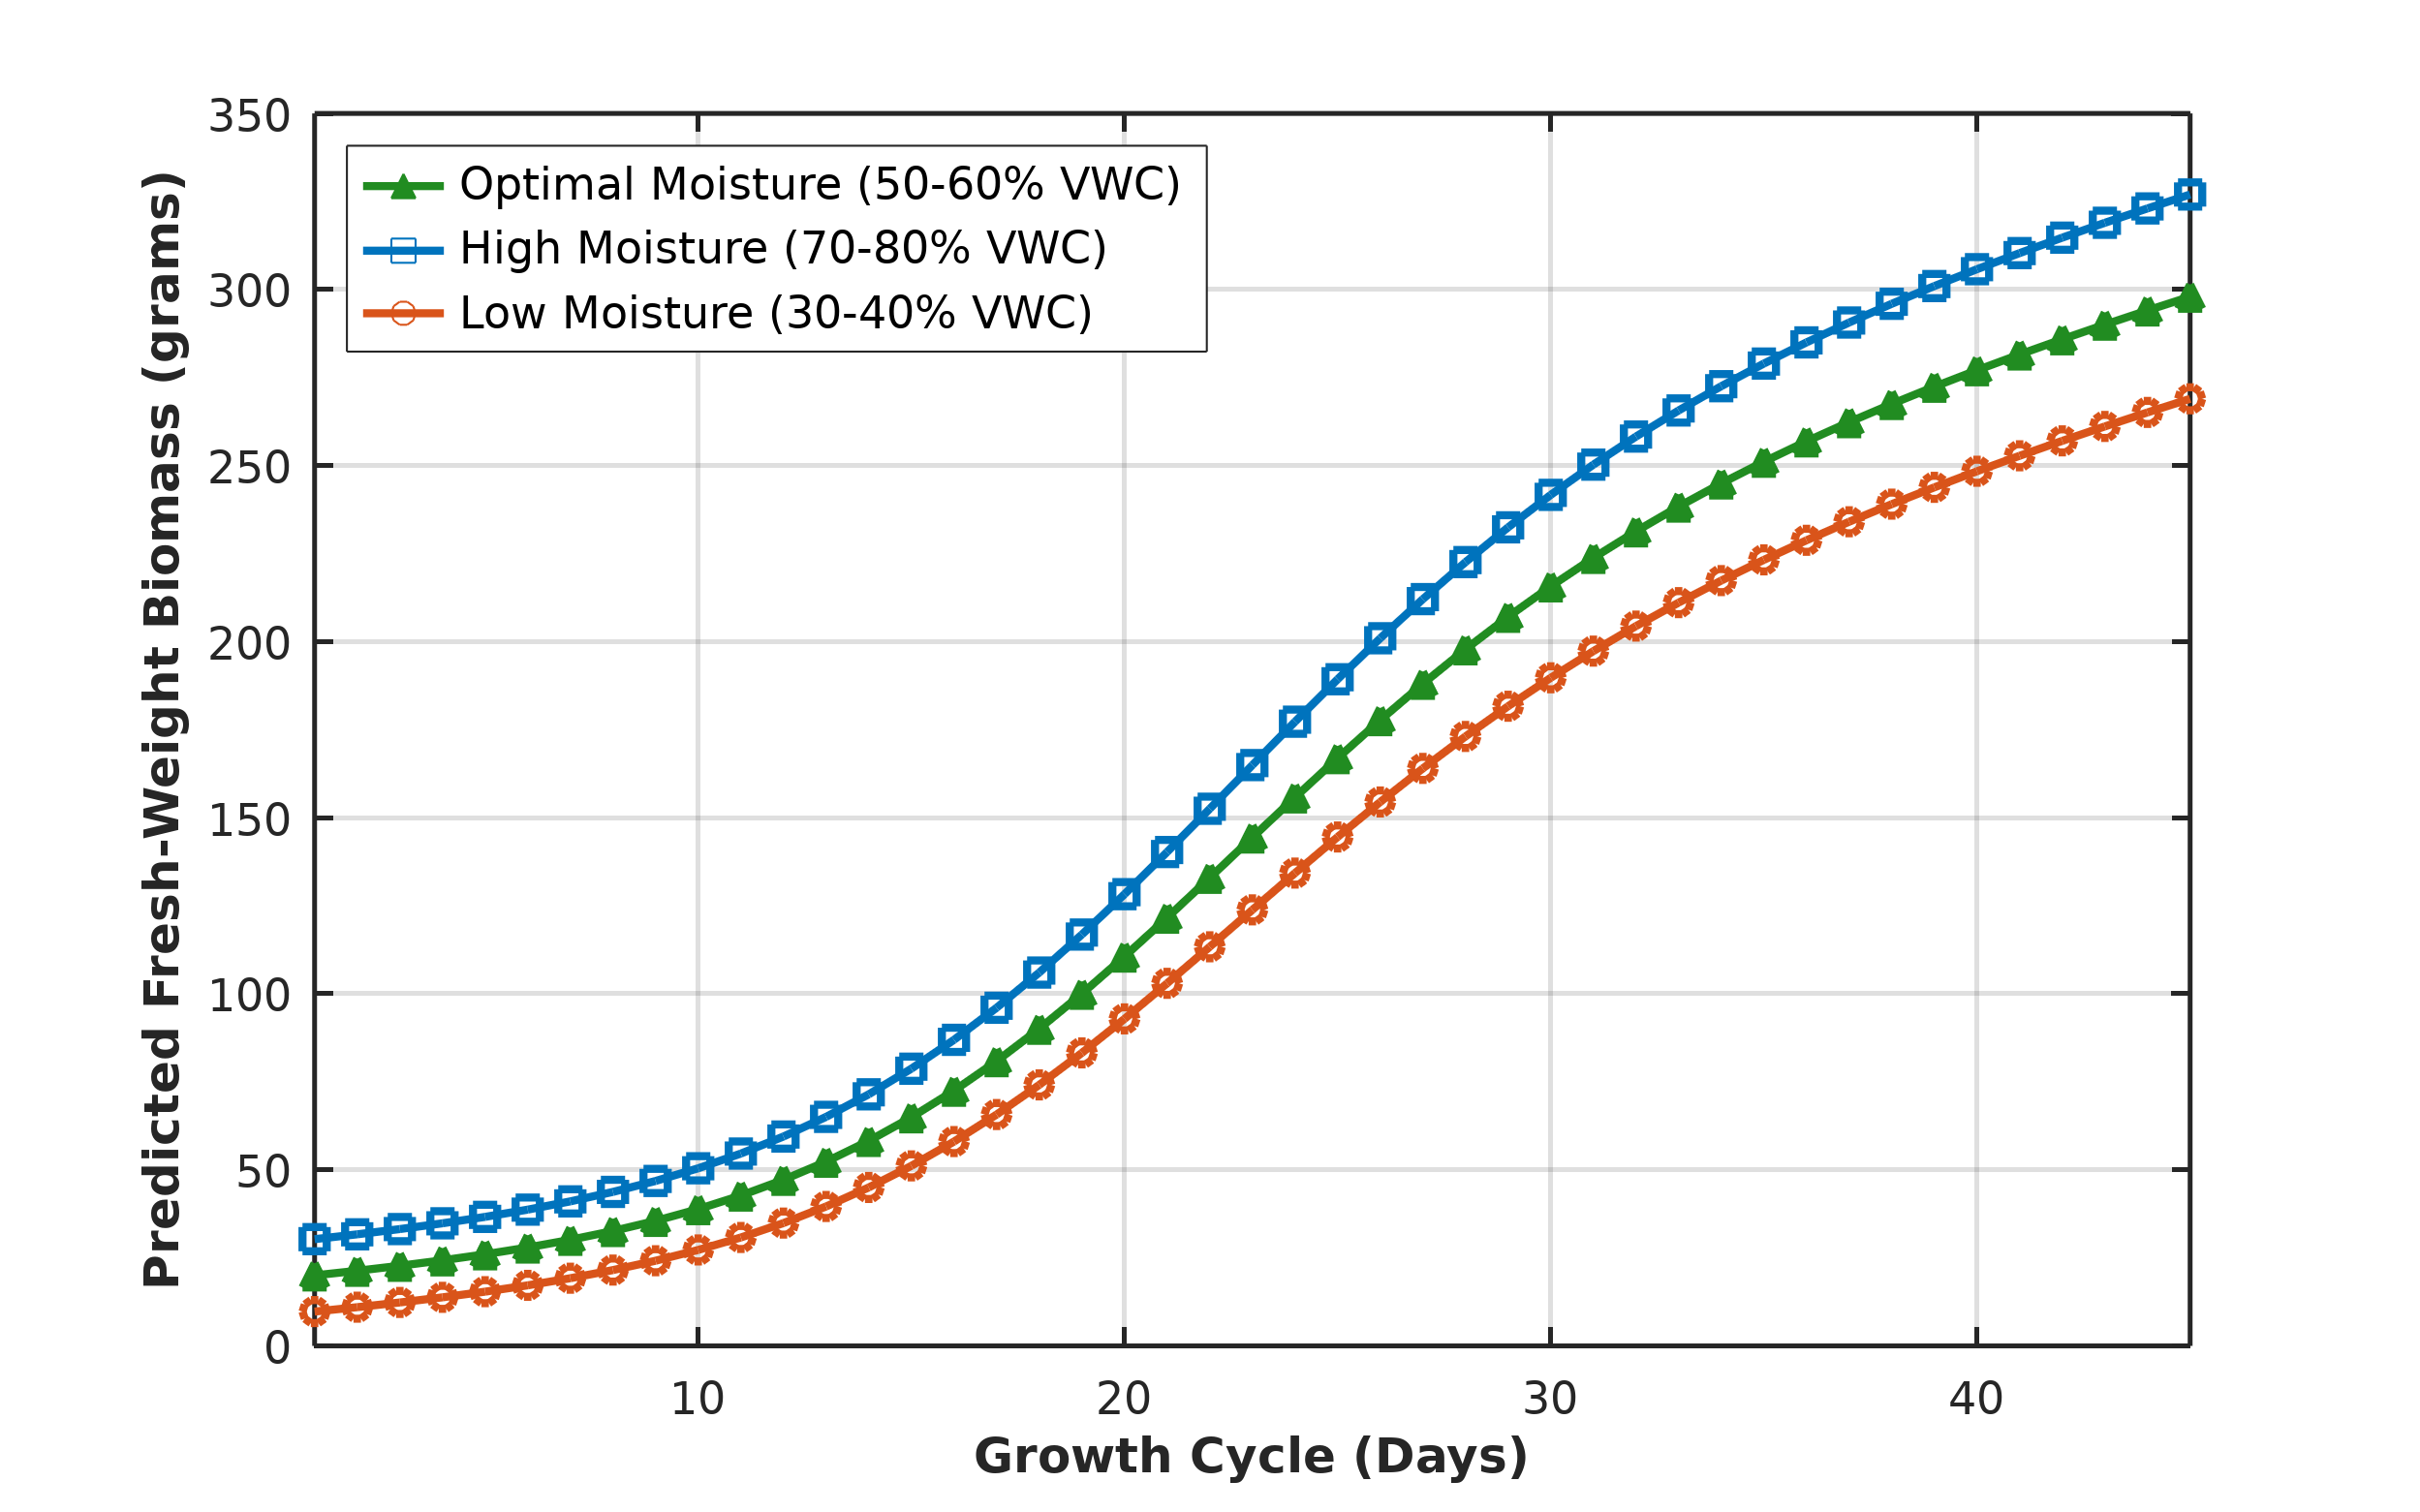
\includegraphics[width=\linewidth]{Predicted_Yield_Curves.png}
    \caption{Simulated multivariate polynomial regression predictions demonstrating Pechay fresh-weight biomass progression across a 35-day cultivation cycle under varying differential soil moisture treatments.}
    \label{fig:yield_curves}
\end{figure}

Because the 35 daily observations within a single plant's time-series are highly autocorrelated, standard validation splitting would artificially inflate model confidence. Therefore, the mathematical predictive integrity of the regression curve is strictly evaluated using Leave-One-Plant-Out Cross-Validation (LOOCV). The model's capacity to explain natural biological variance is assessed using the coefficient of determination (\(R^2\)):

\begin{equation}
R^2 = 1 - \frac{\sum (Y_{\text{actual}} - \hat{Y})^2}{\sum (Y_{\text{actual}} - \bar{Y})^2}
\tag{2}
\end{equation}

Concurrently, the Mean Absolute Error (MAE) quantifies prediction error scale parameters in physical mass units:

\begin{equation}
\text{MAE} = \frac{1}{m} \sum_{i=1}^{m} |Y_{\text{actual}, i} - \hat{Y}_i|
\tag{3}
\end{equation}

where \(m\) represents the total number of harvested plant validation specimens evaluated during LOOCV.

\section{Electrical Power Configuration Profile}

To address non-functional constraints regarding structural deployment feasibility, the system's electrical operational configurations are documented. The baseline telemetry layer operates on a standard \(3.3\mathrm{V}\) logic rail, with the ESP32-S3 demanding approximately \(80\mathrm{mA}\) during deep-sleep polling states and peaking at \(240\mathrm{mA}\) during localized solenoid valve actuation.

The image processing computer vision layer operates on a \(5\mathrm{V}\) rail. By transitioning from a hard-cycled power model to a \texttt{cron}-scheduled always-on architecture, the Raspberry Pi Zero 2W draws a continuous idle current of approximately \(100\mathrm{mA}\) to \(150\mathrm{mA}\). During the brief 60-second daily active imaging window, current draw peaks at \(350\mathrm{mA}\). This constant-power configuration ensures file-system stability and reliable script execution, resulting in an estimated total daily power footprint of 12 to 18 Watt-hours (Wh). This minimal energy profile validates the architecture's continued viability for resource-limited urban residential environments.

\subsection{Power Failure Mitigation}

To address the risk of power interruptions—which are common in tropical urban environments—the system implements a multi-layer mitigation strategy following the approach validated by Aala et al. (2022) in their precision urban farming system \cite{Aala2022}.

First, the Raspberry Pi Zero 2W and ESP32-S3 are powered through an uninterruptible power supply (UPS) with pass-through charging capability. Using an APC Back-UPS 650 or equivalent 12V, 7Ah UPS, the system provides approximately 4 hours of continuous runtime for the full architecture, which is sufficient for most short brownouts in urban residential settings.

For outages exceeding the UPS battery capacity, the system relies on software recovery mechanisms. The Raspberry Pi performs a graceful shutdown when the UPS battery level drops below a critical threshold, preventing SD card corruption that would otherwise result from sudden power loss. The ESP32-S3 continues to operate independently, drawing minimal current to log sensor data and maintain irrigation schedules for up to 48 additional hours. Furthermore, the ESP32 stores current soil moisture readings and irrigation state in non-volatile memory using the Preferences library. Upon power restoration, the ESP32 reads the last saved state and resumes normal operation without overwatering or underwatering the plants.

A startup script on the Raspberry Pi checks the timestamp of the last successful image capture upon boot. If the daily capture was missed due to a power outage during the scheduled 12:00 PM capture window, the script executes the GPR pipeline immediately, ensuring that a daily reading is not skipped. Any missed days are flagged in the anomaly log and interpolated using the 3-day centered moving average. This layered approach—hardware backup, graceful degradation, state recovery, and automated resume—ensures data integrity and system reliability throughout the 35-day grow-out cycle.

%=============================================================================
%  ADDED NOVEMBER 2026. The sections below describe the system AS BUILT.
%  The sections above describe the system AS PROPOSED and still contain the
%  figures listed in the deviation table. Reconcile them during the rewrite
%  pass: where the two disagree, the as-built description is correct.
%=============================================================================

\section{Enclosure and Electronics Housings}
\label{sec:enclosures}

The deployed station is housed in a timber-framed greenhouse enclosure erected
on the approved campus site. The frame is built from 1.5-inch nominal timber
members rather than the half-inch PVC of the first prototype, which flexed at
the joints once standing at full height and could not carry the roof load. A
pitched roof section in PVC pipe is fastened to the frame by custom
3D-printed PLA clip-ons secured with screws, and the structure is covered with
a 200 by 200\,cm ultraviolet-stabilised plastic sheet over four mesh net
panels of 120 by 60\,cm.

Three enclosures were designed in CAD and printed in-house to carry the
electronics. All were modelled by Cedric Tan.

\subsection{Tiered Actuator Enclosure}

The actuating hardware is carried in a three-tier stacked enclosure, shown
assembled in Figure~\ref{fig:cad_actuator}. Each tier is an open frame with
integrated mounting bosses, and the tiers are separated so that cabling runs
vertically between levels rather than across them. The allocation is as
follows: the top level carries the ESP32-S3 controller board and the relay
banks, the middle level carries the pump and four solenoid valves, and the
bottom level carries the remaining five valves.

\begin{figure}[ht]
\centering
\begin{tabular}{ccc}
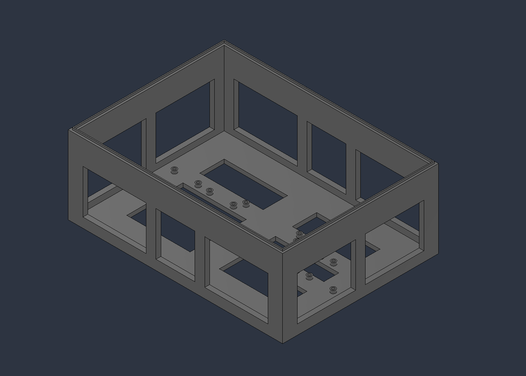
\includegraphics[width=0.30\linewidth]{cad_tier1.png} &
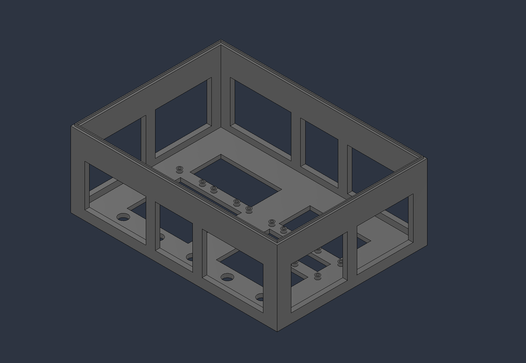
\includegraphics[width=0.30\linewidth]{cad_tier2.png} &
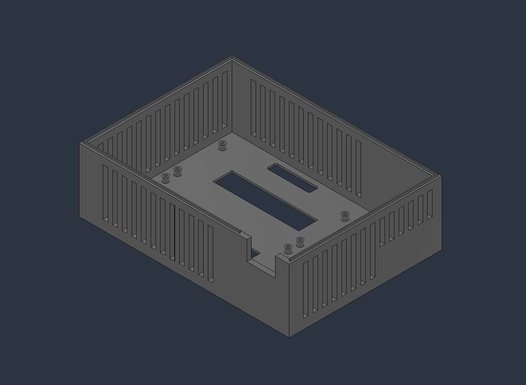
\includegraphics[width=0.30\linewidth]{cad_tier3.png} \\
(a) First tier & (b) Second tier & (c) Third tier \\
\end{tabular}
\caption[CAD models of the three actuator enclosure tiers]{CAD models of the
three tiers of the actuator enclosure. The third tier carries louvred side
walls for convective ventilation.}
\label{fig:cad_tiers}
\end{figure}

\begin{figure}[ht]
\centering
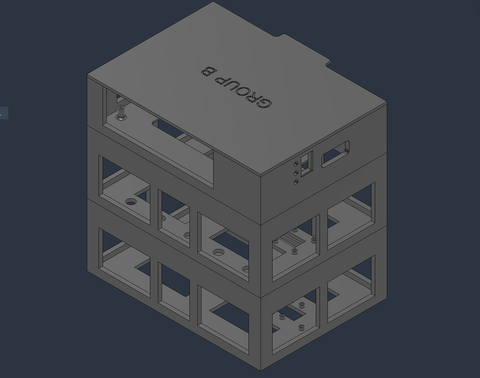
\includegraphics[width=0.5\linewidth]{cad_actuator_assembly.png}
\caption[Assembled tiered actuator enclosure]{The three tiers assembled with
the lid fitted.}
\label{fig:cad_actuator}
\end{figure}

Raising the assembly off the ground on its own structure, rather than seating
it directly on the soil beside the array, was a deliberate choice. The station
operates outdoors through the wet season, and splash and runoff at ground level
are the most likely route for water to reach the relay contacts.

\subsection{Camera and Controller Housing}

The Raspberry Pi Zero 2 W and the Camera Module 3 share a single vented
enclosure clamped to the PVC roof pipe directly above the array.
Figure~\ref{fig:cad_pi} shows the internal arrangement and the assembled
housing.

\begin{figure}[ht]
\centering
\begin{tabular}{cc}
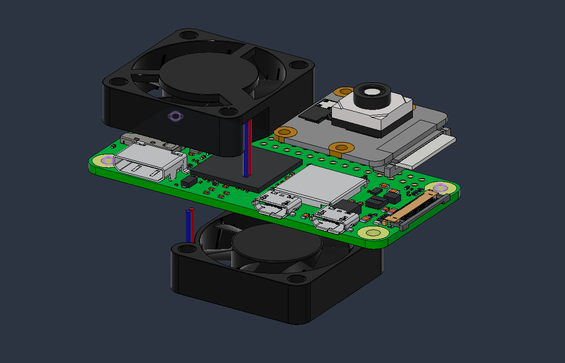
\includegraphics[width=0.46\linewidth]{cad_pi_interior.png} &
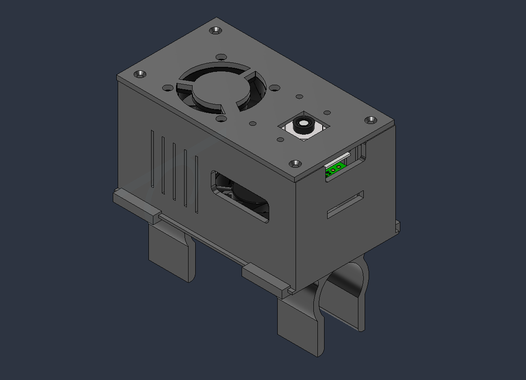
\includegraphics[width=0.46\linewidth]{cad_pi_enclosure.png} \\
(a) Internal arrangement & (b) Assembled housing \\
\end{tabular}
\caption[CAD model of the camera and controller housing]{CAD model of the
camera and controller housing. The exploded view shows the single-board
computer with the camera module mounted to it and a cooling fan above and
below; the assembled view shows the camera aperture, the fan grille, the
louvred vents and the clip mounts that fix the housing to the roof pipe.}
\label{fig:cad_pi}
\end{figure}

Fixing the camera to the structure rather than standing it beside the array
holds the viewpoint constant between daily captures, which the measurement
depends on: the per-pot measurement areas are defined in image coordinates, so
any movement of the camera displaces every region at once.

\section{Summary of Deviations from the Proposed Design}
\label{sec:deviations}

Table~\ref{tab:deviations} records every respect in which the deployed system
differs from the design set out in the approved proposal, together with the
reason. It is given in full because several of the deviations affect how the
results of Chapter~\ref{chap:results} must be read.

\begin{table}[ht]
\centering
\caption{Deviations of the deployed system from the approved proposal}
\label{tab:deviations}
\footnotesize
\begin{tabularx}{\linewidth}{lXX}
\toprule
\textbf{Item} & \textbf{As proposed} & \textbf{As built} \\
\midrule
Growing medium & Commercial potting mix from the Department of Agriculture &
Garden soil, rice hull and vermicast at 8:4:3, batch-mixed so every pot
receives identical substrate \\
Container & 200\,mm upper diameter, approximately 3.0\,L &
130\,mm diameter \\
Camera & Raspberry Pi Camera Module V2 &
Camera Module 3 (imx708), captured at 1296 by 1296 px, two-times binned from
4608 by 2592 \\
Illumination & Fixed overhead LED array for standardised illumination &
Natural light only. Exposure is normalised to a target mean brightness at each
capture, with gain and white balance locked \\
Enclosure & PVC-framed structure & Timber-framed structure with a PVC roof
section, after the PVC frame failed under roof load \\
Canopy measure & Green Pixel Ratio over a fixed circular region of interest &
Green Pixel Ratio over a non-overlapping per-pot area bounded at 175\,px,
after the fixed circle returned zero for living plants that leaned past the
pot rim \\
Hue threshold & Expressed in degrees &
Hue 38 to 85 in OpenCV units on a 0 to 179 scale, with saturation at least 100
and value at least 55 \\
Morphological filter & Not specified &
3 by 3 opening, sized from a physical limit of 2.2\,mm at
1.34\,px\,mm$^{-1}$ \\
Controller power & ESP32-S3 polling from deep sleep at 80\,mA &
Always-on architecture, mains supplied through an uninterruptible power supply \\
Cycle length & 35 days & 30 days \\
\bottomrule
\end{tabularx}
\end{table}

\section{Validation of the Canopy Measurement}
\label{sec:gpr_validation_method}

The calibration procedures of Section~\ref{sec:calibration} establish that the
apparatus functions: that the probes read correctly, that the capture fires on
schedule, that the regions fall on the pots. None of them establishes that the
Green Pixel Ratio corresponds to the canopy an observer would identify. That
is a separate question, and it is answered by the procedure set out here.

Noon frames are selected from the capture series and each pot image within
them is annotated independently by two labellers, who mark the leaf blades
only, excluding stems, shadow and soil. Each manual mask is compared with the
automatic mask pixel by pixel, yielding true positives, false positives and
false negatives, from which precision, recall, Intersection over Union and the
Dice coefficient are computed. The Green Pixel Ratio derived from each manual
mask is compared with the automatic value to give the measurement bias and the
limits of agreement by the Bland-Altman method.

The two manual masks are additionally compared with each other. This step is
essential rather than supplementary: it establishes the agreement that two
trained humans achieve on the same images, and it is that figure, not unity,
against which the algorithm must be judged. Leaf boundaries in an overhead
image carry an irreducible ambiguity, and an algorithm cannot reasonably be
required to exceed the consistency of the observers defining the ground truth.

The procedure is implemented in \texttt{Dual\_Archi/tools/gpr\_validate.py}
and its results are reported in Section~\ref{sec:gpr_validation}.
